\chapter{Cheguei agora no vento}

\section{O discurso se espalha}


\singlespacing
\begin{flushright}
\textit{``Amor}

\textit{Vim te buscar}

\textit{Em pensamento}

\textit{Cheguei agora no vento''}

Walter Franco

\end{flushright}
\doublespacing


\textbf{``A toda hora e a todo momento''}

Cena 1, Julho de 2005, Oxford, Reino Unido.

Jimmy Wales é convidado ao palco para realizar sua apresentação de 20 minutos no TEDGlobal 2005, primeira edição deste \textit{spin off} das TED Conferences, criado para ``\textit{dar um foco ainda mais forte em ideias realmente grandes para mudar o mundo: memes e sonhos de imbricações de mundos da ciência, arquitetura, tecnologia, negócios e organizações sem fins lucrativos, criatividade global e ingenuidade local}'' \citep{ted_global_2005}.\footnote{No original: ``\textit{even stronger focus on really big world-changing ideas: memes and dreams from the intersecting worlds of science, architecture, technology, business and nonprofit, global creativity and local ingenuity}''.  https://www.ted.com/about/conferences/past-teds/tedglobal-2005 , acessada em 19 de março de 2020.}

A palestra acontece um ano após Wales, ou Jimbo, como é conhecido o fundador mais famoso da Wikipédia dentre seus/suas colegas enciclopedistas, falar em uma entrevista a frase que ele utiliza para abrir a apresentação:\footnote{Palestra disponível em https://www.ted.com/talks/jimmy\_wales\_the\_birth\_of\_wikipedia?language=en , acessada em 19 de março de 2020.}

``\textit{Imagine um mundo onde a toda pessoa do planeta é oferecido acesso livre/gratuito à soma de todo conhecimento humano. É isso que estamos fazendo.}'' \citep{wales_interview_2004}\footnote{Tradução livre. No original: ``\textit{Imagine a world in which every single person on the planet is given free access to the sum of all human knowledge. That's what we're doing.}'' Optamos por traduzir ``\textit{free}" como livre/gratuito pois ambos os sentidos estão presente no uso da palavra neste contexto. }

Em seguida, ele detalha o funcionamento da Wikipédia, explicando que ela é uma enciclopédia em licença livre, feita por milhares de voluntários de todo mundo em vários idiomas, e utiliza um software wiki, um tipo de ferramenta onde \textbf{qualquer um/a pode rapidamente editar}\footnote{ Nesta seção todos os grifos são do autor.} e salvar, com sua alteração indo ao ar para toda a internet imediatamente \citep{wales_birth_2005}.

A apresentação então detalha como a enciclopédia é mantida totalmente por voluntários/as, e que a \textit{Wikimedia Foundation} (WMF), organização sem fins lucrativos criada por Wales para manter a Wikipédia, acabara de contratar seu primeiro e único funcionário em janeiro de 2005, um desenvolvedor de software. É mencionado que o custo de 5 mil dólares com internet é praticamente o único que a organização tem para se manter ativa.

Wales então explica que praticamente não existem controvérsias na escrita de conteúdos na Wikipédia, devido ao fato dos/as editores/as entenderem e respeitarem a política editorial da neutralidade. E conta que as poucas controvérsias que emergem são rapidamente resolvidas, pois não se discutem nem suas verdades  nem suas objetividades, bastando aos/às editores/as relatarem o que os diferentes lados respeitáveis acham da contenda, sem que a enciclopédia precise tomar partido de nenhum deles. A explicação sobre a forma dos/as wikipedistas resolverem controvérsias se encerra com Wales afirmando que esta metodologia funciona pois a comunidade é muito diversa, com membros/as de diferentes origens políticas, religiosas e culturais.

\textbf{Cena 2, Junho de 2015. São Paulo, Brasil.}

Um dos mais de 100 funcionários da WMF participa de uma reunião com voluntários/as interessados/as em criar uma organização no Brasil focada em atividades de extensão do Movimento Wikimedia, nos mesmo moldes de dezenas de outras criadas pelo mundo e financiadas pela WMF, motivados/as pelo fato de que, \textbf{apesar de todos/as poderem editar, poucos/as brasileiros/as editam a Wikipédia}.

Esta é a quarta vez que um grupo tenta criar um ``capítulo Wikimedia''\footnote{No Movimento Wikimedia, capítulos são organizações satélites espalhadas pelo mundo. Esta estrutura será explicada em nosso capítulo 3.} no Brasil, depois das três primeiras fracassarem por atritos, diferenças de visão e impossibilidade de membros da comunidade de trabalharem em conjunto.

Após falar sobre o interesse da Fundação em aumentar a diversidade de seus/suas editores/as, especialmente engajando mais moradores/as do chamado sul global, o funcionário da WMF distribui seu cartão de visitas, onde pode ser lido no verso: ``\textit{Imagine um mundo onde todo ser humano pode compartilhar  livremente/gratuitamente a soma de todo o conhecimento. Este é o nosso compromisso}'' (veja figura \ref{fig:cartao_wmf}).\footnote{Tradução livre. No original ``\textit{Imagine a world in which every single human being can freely share \textbf{in} the sum of all knowledge. That’s our commitment}''. Destacamos o uso do ``\textit{in}'' após o ``\textit{share}'', que passa uma ideia de compartilhamento ativo e por dentro, que é perdida em nossa tradução para o português.}

\begin{figure}[H]
    \centering
    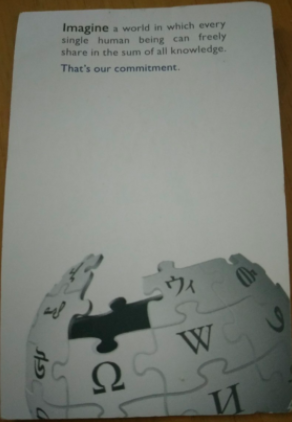
\includegraphics[width=.4\textwidth]{Images/cartao_wmf.png}
    \caption{Verso do cartão de visitas dos funcionários da Wikimedia Foundation.}
    \label{fig:cartao_wmf}
\end{figure}



\newpage

\section{A realidade confunde}

\singlespacing
\begin{flushright}
\textit{``Eu só voltei}

\textit{Pra te contar}

\textit{Viajei}

\textit{Fui pra Serra do luar}

\textit{Eu mergulhei}

\textit{Ah, eu quis voar}

\textit{Agora vem}

\textit{Vem pra terra descansar''}

Walter Franco

\end{flushright}
\doublespacing

\subsection{Para onde vai um conteúdo reprovado?}

\textbf{Cena 3, Abril de 2017.\footnote{Cena escrita a partir de entrevista realizada com Alberto Lima no Rio de Janeiro, no dia 06 de fevereiro de 2020. Quando não explicitamente atribuídas a outrem, todas as aspas desta sessão são falas do entrevistado.} Rio de Janeiro.}

O engenheiro Alberto Lima, professor do curso técnico em Eletrônica do CEFET/RJ, liga seu computador decidido a criar o verbete ``Andes-SN'' na Wikipédia, para falar sobre o Sindicato Nacional dos Docentes das Instituições de Ensino Superior.

Concursado em 2011, Alberto participou ativamente do movimento grevista de 2012, greve esta deflagrada pelas bases em assembleia, contrariando indicação das direções sindicais. Após integrar o comando local de greve, inclusive participando de grandes atos em Brasília/DF, Alberto se junta a companheiros/as paredistas em 2013, concorre, e ganha a eleição para a direção da Adcefet-rj, seção sindical do Andes em sua instituição.

Ao final de sua gestão como presidente do sindicato local, em 2017, Alberto acreditava que o Andes-SN, apesar de ser um dos maiores sindicatos do Brasil, com seções em todas as universidades federais, não possuía uma grande presença digital. Resolveu ler sobre boas práticas de criação de verbetes na Wikipédia e, apesar da dica encontrada de começar editando artigos pré-existentes ao invés de criar um novo do zero, sentiu-se preparado para criar um verbete. Pesquisou se existiam artigos sobre outras entidades similares à sua, e se lembra de ter encontrado vários, ``\textit{alguns inclusive bem curtos com apenas uma referência}''. Com sua pesquisa feita, sentiu-se confiante e começou a escrever sobre seu sindicato nacional.

O professor nos conta que começou a escrever direto na página da Wikipédia. Fez um texto longo, ``\textit{que tinha inclusive uma ligação interna}'', duas referências e estruturado com ``\textit{Introdução} e "\textit{contextualização}''. Se sentia seguro e confortável ao escrever alí, pois afinal ``\textit{qualquer um pode editar a Wikipédia}''.
	
Sabia que seu texto ``\textit{não estava completamente redondo}'', mas resolveu salvar como estava para continuar mais tarde. Nosso editor novato nos conta que já tinha visto alguns verbetes na Wikipédia marcados com avisos como ``\textit{esboços}'', ``\textit{demandando estruturação}'' ou ``\textit{carece de referências}'', e sabia que a mesma coisa poderia acontecer com seu verbete, que seria melhorado mais tarde.

Porém, alguns segundos depois ele é surpreendido por uma notificação informando que seu artigo havia sido removido pelo administrador EVinente, atendendo a um pedido de outro usuário. Ao acessar o endereço da página, se deparou com a seguinte imagem:

\begin{figure}[H]
    \centering
    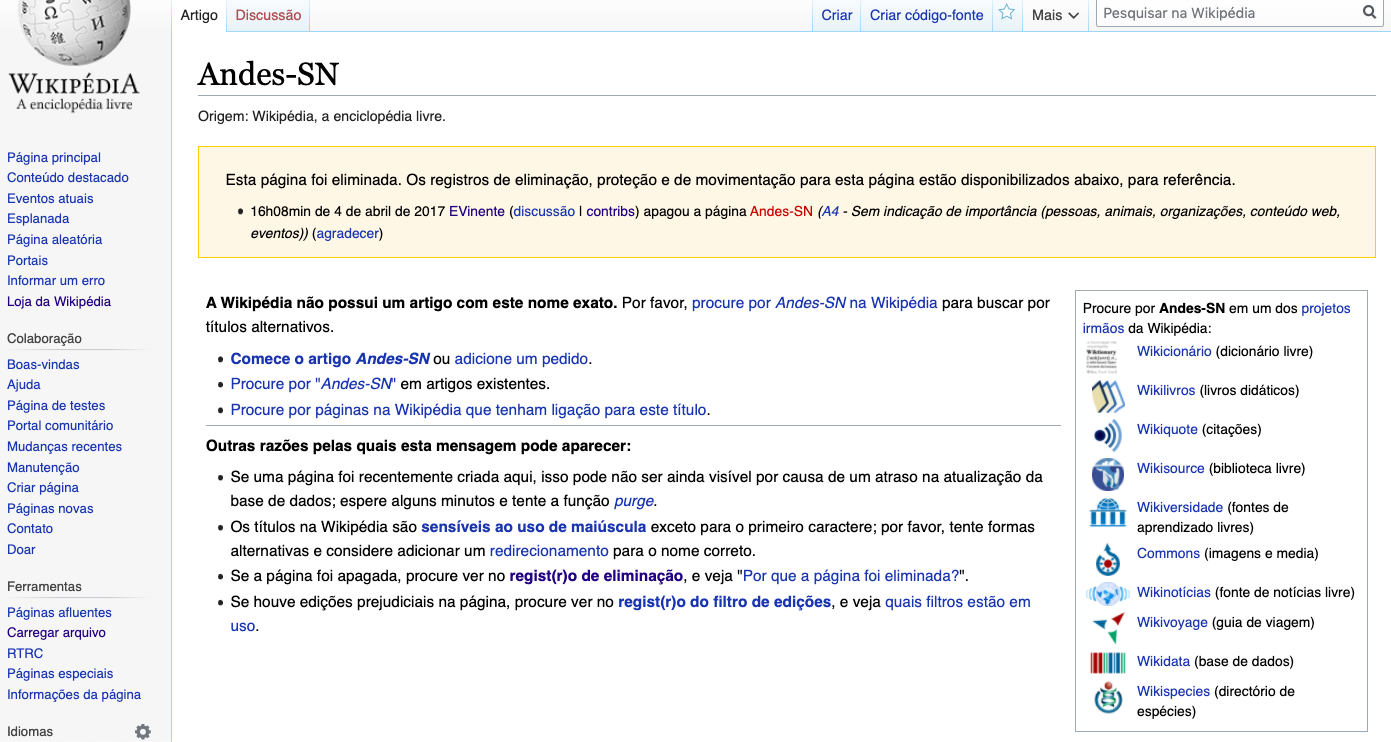
\includegraphics[width=1\textwidth]{Images/andes.png}
    \caption{Verbete Andes-SN com aviso de eliminação.}
    \label{fig:verbete_andes}
\end{figure}

Lembrando das apresentações assistidas nos seminários de pesquisa sobre controvérsias na Wikipédia, Alberto vai à página de discussão do usuário que solicitou a eliminação, onde o profesor então explica saber que o verbete ainda não estava ideal, que teria mais referências para adicionar (``\textit{notícia de greve é o que mais tem}''), inclusive com uma tese acadêmica sobre a história do sindicato. Concluiu informando que gostaria de continuar editando.

\begin{figure}[H]
    \centering
    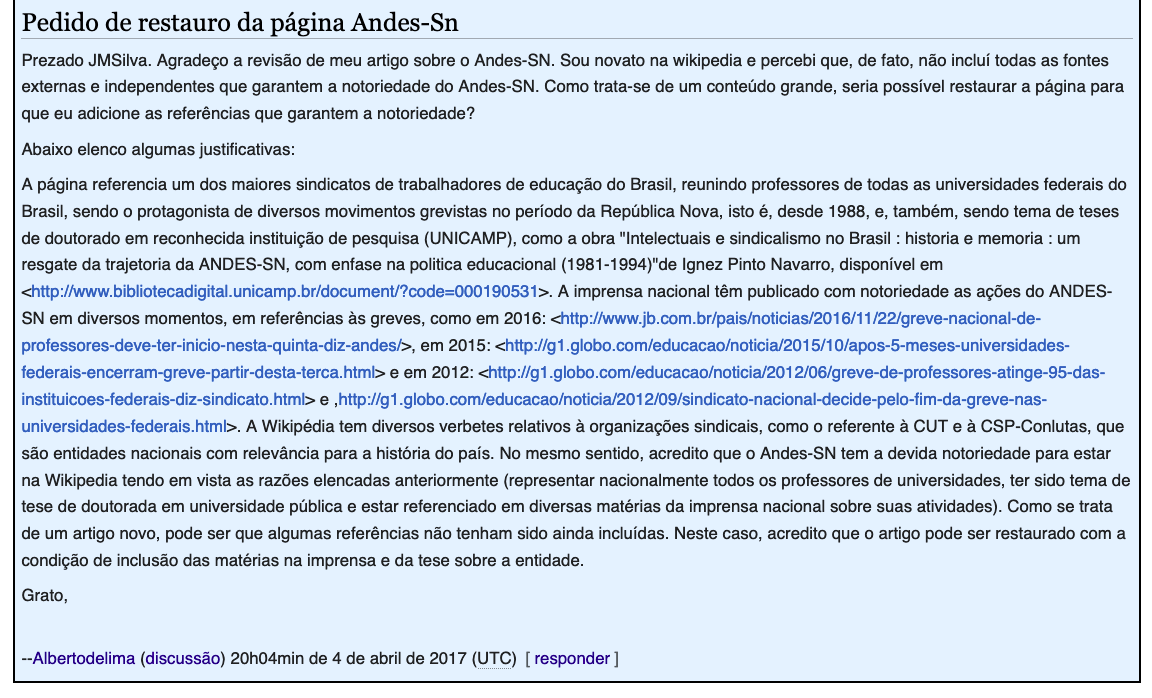
\includegraphics[width=1\textwidth]{Images/alberto-pedido-restauro.png}
    \caption{Página "Wikipédia:Pedidos/Restauro" com o pedido de Albertodelima para que a solicitação remoção feita por JMSilva fosse revista.}
    \label{fig:pedido_restauro_andes}
\end{figure}


O Diálogo então, segundo a memória de nosso protagonista, seguiu mais ou menos assim:

-Se você já sabia onde encontrar mais referências por que não as colocou logo?

-Eu estava sem tempo, mas vou colocar. Porém, o que eu já escrevi sumiu. Quero editar e melhorar, mas não tenho backup.

- Você vai ter que escrever tudo de novo.

Alberto, traído pela confiança na ferramenta, não seguiu sua prática corriqueira de escrever offline e depois "copiar e colar" o conteúdo criado em uma ferramenta online, e agora se via sem possibilidade de acessar novamente sua criação, eliminada do histórico público da Wikipédia.
Como resultado, ele, que estava ocupado com a reta final de seu mandato à frente da Adcefet-rj e já cursando doutorado, resolveu abrir mão de disputar a construção de conteúdos na Wikipédia. ``\textit{Eu nunca mais criei nenhum outro artigo. Nem esse.}''

No início de 2020, Alberto ficou feliz em ver que fora criado em 2018 outro verbete sobre o Andes-SN, desta vez levando seu nome completo, ``Sindicato Nacional dos Docentes das Instituições de Ensino Superior''. Apesar do novo verbete ser muito inspirado na seção ``Sobre'' da página sindicato, não apresentar nenhuma referência, ser muito menos acadêmico que o anterior, e de ter recebido as marcações de ``\textit{Este artigo não cita fontes confiáveis e independentes}'' e ``\textit{Este artigo é um esboço}'', em nenhum momento foi ``proposto para eliminação''.
\newpage
\subsection{Engajamentos e desengajamentos}

\textbf{Cena 4, Janeiro de 2016. Niterói, Brasil.\footnote{Cena escrita a partir de entrevista realizada com Carlos Eduardo Mattos da Cruz no Rio de Janeiro, no dia 06 de fevereiro de 2020. Quando não explicitamente atribuídas a outrem, todas as aspas desta sessão são falas do entrevistado.}}

Carlos Eduardo Mattos da Cruz, responsável pela criação de cursos para os telecentros do município\footnote{Espaços criados para o desenvolvimento de atividades educacionais complementares pelo Programa Niterói Digital, desenvolvido pela Secretaria Municipal de Educação, Ciência e Tecnologia de Niterói.}, orgulhosamente recebe o coordenador do Wiki Educação Brasil, grupo local reconhecido pela Wikimedia Foundation, para iniciar o curso de capacitação de professores/as da rede municipal no uso dos projetos Wikimedia, seguindo a proposta dos telecentros de oferecer uma ``\textit{educação contemporânea sem a ditadura do MEC}''.

O projeto desta formação foi desenvolvido por Cadunico, como Carlos gosta de se apresentar, a partir de conversas com funcionários da Wikimedia Foundation, que contaram-lhe sobre como os projetos educacionais com a enciclopédia só aconteciam em universidades, e que havia o desejo de diversificar o perfil dos editores e levar a prática de escrita wiki para outros níveis educacionais.

Cadunico decidiu tocar o projeto mesmo tendo experiências pessoais não agradáveis no mundo das wikis. Em julho de 2012, criara um verbete sobre o Gnugraf, maior evento de softwares livres para edição gráfica da América Latina, organizado por ele e por sua esposa Cléo Mattos. Pouco tempo depois, foi surpreendido com a remoção do verbete. Através do apoio de amigos que trabalhavam para o movimento e de um editor experiente, conseguiu, ``\textit{depois de muito sufoco}'', deixar no ar uma versão bem simplória do texto original. Até hoje Cadunico tem receio de editar o verbete e adicionar mais informações, para não ``\textit{chamar a atenção}'' de revisores, que podem novamente decidir apagá-lo, assim como aconteceu com sua página de usuário.

Foi em maio de 2013 que ele teve sua página de usuário apagada na Wikipédia. Em suas palavras, ``\textit{porque coloquei mais um item em uma lista de coisas que eu já tinha feito e um robô bloqueou a página}''. Curiosamente, ao observarmos o histórico da página, vemos que a ação não havia sido realizada por um robô, e sim por um dos usuários humanos mais ativos da Wikipédia lusófona. Perguntado sobre mensagens recebidas em sua página de discussão, Cadunico disse desconhecer tal ferramenta, e emendou: ``\textit{quando entro no Facebook pela primeira vez ele tem umas setinhas e umas formas de mostrar onde estão as coisas. Não me lembro de ter visto isso quando me cadastrei na Wikipédia. Só utilizei a 'caixa de areia'\footnote{Área da Wikipédia onde editores podem realizar testes.} por que eu já tinha conversado com pessoal da fundação que me falou dela. Mas ainda assim, a gente escreve lá e ninguém lê. Ninguém te dá dicas sobre o que melhorar antes de enviar conteúdo para o artigo}''.

Após frustrar-se com a Wikipédia, Cadunico ``se muda'' para o Wikilivros, projeto do Movimento Wikimedia para escrita de livros didáticos. Consegue com sucesso criar uma apostila para utilização do software de diagramação \textit{Scribus}\footnote{Apostila disponível em  https://pt.wikibooks.org/wiki/Apostila\_de\_Scribus , acessada em 30 de março de 2020.}, retomando assim sua confiança na possibilidade de trabalhar em conjunto com o movimento.

Então, em 2015, Caudnico convidou representantes do Movimento Wikimedia, que trabalhavam em conjunto com a Fundação, para serem responsáveis pela formação dos/as professores/as. Acreditou que essa chancela evitaria que situações desagradáveis como as vividas por ele na Wikipédia se repetissem. ``\textit{Eu queria botar nos telecentros o símbolo da Wikimedia, e falar que aqui é um núcleo oficial, com aula dada pelo pessoal da própria Fundação. Fizemos banners e tudo mais}''.

A meta do projeto era fazer com que professores da rede municipal de Niterói adotassem ferramentas wiki em suas práticas pedagógicas. A ideia era o/a professor/a editar em suas horas fora de sala de aula, bem como editar com seus/suas alunos/as. Para além da Wikipédia, eles/elas seriam estimulados a escrever livros didáticos em conjunto no Wikilivros e inclusive a compartilhar seus planos de aula no Wikiversidade. O projeto ainda previa, em um segundo momento, expandir a capacitação para a Secretaria de Turismo, que poderia ajudar a manter verbetes na Wikipédia sobre a cidade de Niterói.

O projeto era grandioso. Contaria com ciclos de dois anos, com um ano de capacitação seguido de um ano com os/as professores/as atuando de forma independente, e no ano seguinte um novo ciclo se iniciaria, com nova formação para reciclagem e aprofundamento. Os encontros aconteciam no Telecentro do Terminal Rodoviário João Goulart. ``\textit{Era o maior telecentro, com a melhor internet e as melhores máquinas}''. Por duas vezes na semana, a equipe de lá parava de atender os outros telecentros (o escritório de gestão de todos os telecentros do município ficava nesta unidade e sua equipe auxiliava no suporte aos telecentros menores) para se dedicar exclusivamente à capacitação Wikimedia.

``\textit{Treinamentos como este começam cheios e terminam vazios. Mas com este foi diferente. Começou cheio e terminou mais cheio ainda.}'' O boca a boca entre os/as professores/as era intenso. Todo dia um/a professor/a ligava perguntando se ainda tinha vaga, e a política da Secretaria de Educação era sempre falar que tinha, para depois se virar em acomodar todo mundo. Um dia Cadunico foi convocado pelo secretário de educação, que queria monitorar o maior problema das capacitações ofertadas no município:

- E aí, como está a evasão?

- Não teve evasão.

- Que bom, então todos os alunos que começaram terminaram?

- Mais ou menos.

- Não estou entendendo.

- Começamos com um aluno por micro, e terminamos com três.

Após um ano de treinamento, era chegado o momento dos/as professores/as criarem conteúdos sem apoio de instrutores experientes. Se aproveitando de práticas de acompanhamento da aplicação dos conteúdos dos cursos com feedback contínuo dos professores, desenvolvidas no projeto "Academia de Jogos", que ensinava a criação de softwares educacionais para crianças e professores, a Secretaria de Educação seguiria então ao longo do ano monitorando de perto a fase do projeto de edição nas wikis.

``\textit{Aconteceu com eles o que aconteceu comigo}'', conta Cadunico. ``\textit{Não era a grande maioria. \textbf{Todos estavam frustrados}. Os professores não conseguiam ter o gosto de ver seus conteúdos publicados}''. Cadunico acrescenta que um professor de história da escola municipal do Fonseca, autor de uma tese acadêmica sobre Niterói antiga, e o mais empolgado durante a capacitação, ``\textit{foi sumariamente censurado e desistiu}''.

E não foram só os professores. Novamente Cadunico se sentiu censurado pelo movimento que ele tanto admirava por ter ``\textit{a missão mais nobre do planeta: a de disponibilizar livre e gratuitamente todo o conhecimento humano}''. Enquanto os professores trabalhavam com as wikis, Cadunico resolveu começar um livro didático no Wikilivros. Um livro de pensamentos que, assim como sua página na Wikipédia, foi apagado. A justificava dada para o apagamento sentensiava que seu material não era considerado um livro didático, sem que Cadunico tivesse recebido qualquer aviso, tentativa de diálogo ou chance de defesa. ``\textit{Um livro de pensamentos não é um livro didático para ensino de português ou literatura? Isso é uma forma de censura. Não deixam explícito que tipo de livro é aceitável ou não, o que já acho errado pois para mim todo livro é aceitável, e simplesmente arrancam seu trabalho, de forma impessoal e muito fria.}''

Independente das frustrações, o projeto seguia o cronograma planejado. Depois de passado meio ano de atividades de escrita wiki sem acompanhamento dos especialistas wikipedistas, a secretaria avisou aos/às professores/as que no início do ano seguinte começaria uma nova turma do projeto, buscando levantar a demanda para realizar seu planejamento. Vários/as professores/as pediram para não acontecer uma próxima versão, solicitando que a secretaria criasse outro projeto, pois eles/as estariam sendo censurados/as e maltratados/as na Wikipédia. ``\textit{Tínhamos conseguido um pequeno exército para editar conteúdos brasileiros, e ele foi se desmotivando e se dissolvendo}''. Perante tantos retornos negativos e nenhum caso de sucesso, o projeto foi cancelado e o segundo ciclo nunca se inicio.

Em paralelo, os telecentros promovíam capacitações de LibreOffice, em parceria com Eliane Domingos e Oliver Hallot, da Associação Libre de Técnicas Abertas (ALTA), parceira local da The Document Foundation\footnote{Organização mantenedora do software LibreOffice.}. Estas capacitações, que formaram mais de 30 mil pessoas, tiveram como contrapartida da equipe de Niterói o compromisso de manter a wiki com a documentação do LibreOffice em português atualizada. ``\textit{O que foi fácil, pois os professores já haviam aprendido a utilizar o MediaWiki nos cursos da Wikimedia}''.

Os/as professores/as de inglês acompanhavam a lista de e-mails dos/as desenvolvedores/as do LibreOffice e passavam para colegas as necessidades de atualização da wiki. A versão em português da documentação era atualizada em tempo real, muitas vezes mais rápido que em inglês. Neste projeto a equipe ficou muito motivada, com professores/as editando inclusive em suas horas vagas, relatando se sentirem úteis e valorizados/as. ``\textit{No LibreOffice ninguém os revertia. Provando que o problema nos projetos Wikimedia não eram ocasionados por falta de qualidade de nossa equipe.}'' \citep{cadunico_2020}
\newpage
\subsection{Comunidade local decisões globais }

\textbf{Cena 5. Junho de 2017. Rio de Janeiro, RJ.}

A disciplina ``Estudos CTS (Ciências-Tecnologias-Sociedades): aproximações brasileiras e latino-americanas'' é ministrada no Programa de Engenharia de Sistemas e Computação da COPPE/UFRJ no 2º período de 2017. A turma é convidada a ler o capítulo 7 do livro ``\textit{Yes, nós temos Pasteur. Manguinhos, Oswaldo Cruz e a história da ciência no Brasil}'' \citep{cukierman_pasteur_2007}, intitulado ``\textit{Prata Preta}''.

``\textit{Chamava-se Horácio José da Silva, mas, que importava?}'' \citep[p. 220]{cukierman_pasteur_2007}. A frase que abre o capítulo citado se refere ao Prata Preta, um personagem da Revolta da Vacina ocorrida no Rio de Janeiro, em 1904, que, como tantos outros tipos, não é encontrado nas narrativas universalizantes da história da ciência brasileira. A leitura, que narra momentos decisivos para a construção sociotécnica das ciências brasileiras pelo ângulo de um personagem que não pensaríamos \textit{a priori} como protagonista, provoca algumas reflexões: a quantos outros/as anônimos/as da história da ciência e tecnologia brasileiras a frase de abertura poderia se referir? Como se faz educação em ciências contextualizada em um país com tantos/as atores/atrizes sem voz? Em espaços populares, fora das salas de aulas dos programas de pós-graduação, quais histórias são contadas e quais versões são aprendidas?

Após a leitura, com todas essas perguntas na cabeça, recebo uma provocação de meu colega de pós-graduação, o doutorando Fernando Severo: ``\textit{vamos melhorar o verbete sobre o Prata Preta na Wikipédia?}''. Imediatamente aceito o convite e vamos analisar o material já existente na enciclopédia. Percebemos então que o verbete biográfico de Prata Preta possuía apenas 1754 bytes\footnote{Unidade de medida utilizada pela comunidade Wikimedia para medir o tamanho de revisões e verbetes.}, sendo a metade deles sobre um bloco de carnaval que leva seu nome.

\begin{figure}[H]
    \centering
    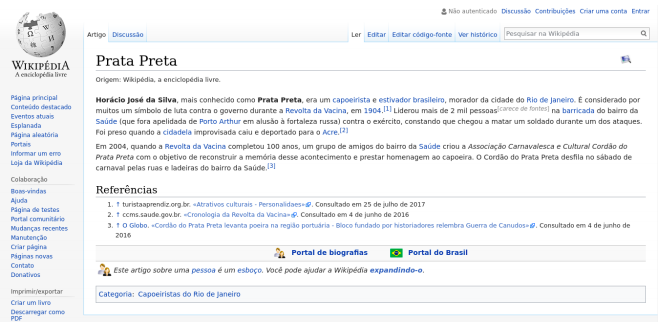
\includegraphics[width=1\textwidth]{Images/pratapreta.png}
    \caption{Versão do verbete Prata Preta encontrado no dia da cena.}
    \label{fig:verbete_pratapreta}
\end{figure}

Aceito o desafio de melhorar o verbete e, enquanto penso sobre os desafios de escrever uma biografia de um subalterno sem voz, com poucas fontes secundárias fiáveis versando sobre sua história, faço uma singela edição com pequenos ajustes ao texto que já estava lá. Para minha grande surpresa, a edição não é salva pela Wikipédia, que me informa: ``\textit{Seu IP está bloqueado}''.

Rapidamente descubro que na verdade não só eu, como milhares de usuários/as da Virtua, maior provedora de internet do Rio de Janeiro, já estavam bloqueados/as por três meses, como resposta a um suposto vandalismo excessivo feito em vários idiomas pelo mesmo range de IP. Essa drástica medida é tomada quando se entende que uma ação orquestrada de vandalismo estará se aproveitando de um provedor de acesso, VPN\footnote{Do inglês Virtual Private Network. São conexões entre máquinas na internet que direcionando o tráfego de uma sempre para a outra.} ou Proxy para mudar de IP constantemente e furar o bloqueio individual a um determinado IP individualizado. E pior, diferente da estratégia de bloqueio simples de IP, onde basta o/a editor/a criar uma conta de usuário/a para (agora rastreado) poder voltar a editar, o bloqueio de faixa de IP incluía também usuários/as registrados/as. Com isso, mesmo meu usuário, com milhares de edições e ficha corrida limpa na enciclopédia, estava proibido de editar.

Fomos então estudar o histórico de edições feitas em nossa faixa de IP e nos surpreendemos com o resultado! Como pode um usuário holandês, que aplicou o bloqueio em todos os sites do Movimento Wikimedia, ter colocado no mesmo balaio de gato Fernando Severo, eu, o IP 179.210.26.120, que estava escrevendo sobre uma escola de samba teresopolitana em português, e o IP 179.210.99.239, que editava sobre a série televisiva ``Meu Pequeno Pônei'' em galego? Não terá seu olhar saxão sido capaz de perceber a distância entre interesses tão distintos e ações de edição? Terá ele conseguido ver apenas uma horda anárquica subdesenvolvida que não tem modos nem educação para escrever uma enciclopédia!?

Saímos então da periferia que é a Wikipédia lusófona e fomos buscar os centros globais de tomada de decisão da enciclopédia. Estudamos as políticas de acesso e de bloqueio globais da comunidade Wikimedia e fomos parar em uma sala de chat em inglês no IRC.\footnote{Do inglês \textit{Internet Relay Chat}, ferramenta para criação de salas de bate papo virtuais.} Lá conversamos com os/as ``gringos/as'', relatando detalhadamente ``o causo'', procurando esclarecê-los a respeito da estrutura do mercado de internet no Rio de Janeiro, com milhões de usuários/as e poucos provedores de acesso; das diversas edições feitas em diferentes wikipédias por editores em nosso range de IP; da forma dinâmica como funciona a distribuição de IP nos provedores de internet; do longo histórico de bom comportamento de meu usuário. Vários/as aliados/as foram convocados/as ao esforço de demonstrar que nosso grupo nada homogêneo, unido involuntariamente por uma faixa de endereços de IP, tem seu valor para a comunidade, e pode ser produtor de conhecimento. Recebi uma desanimadora resposta burocrática de um anglófono, que simplesmente mandou enviar e-mail para um determinado endereço e esperar por um resposta sem prazo.

Mas, eis que de onde parecia que não surgiria mais alento, emerge a empatia de um \textit{steward}\footnote{No Movimento Wikimedia são usuários com permissões para administrar todas as wikis de todos os projetos.} falando português. Ele se solidariza com nosso pleito e nos autoriza a participar novamente do jogo global de construção de conhecimentos na wiki universal, relaxando parcialmente o bloqueio. Agora, após nossa expedição exploratória da implementação da política de bloqueios globais do Movimento durar toda a madrugada, poderíamos novamente editar, desde que estivéssemos devidamente registrados no site com um usuário próprio. Usuários/as anônimos/as continuariam impedidos/as de editar. Afinal, nosso pleito ``tinha seu valor sim, mas também não era para tanto, né?''. Com a confirmação de que havíamos conseguido superar a pane, compondo um novo arranjo suficiente para estabilizar o funcionamento da Wikipédia para nossos usuários, fomos dormir às 5 horas da manhã, sem realizar nenhuma edição no verbete de Prata Preta.

\section{A pesquisa se materializa}

Abrimos este trabalho com cinco cenas, mas poderiam ter sido apresentadas centenas outras em torno da mesma temática. Cotidianamente a Wikipédia convive com esta dicotomia entre ser aclamada como o maior projeto de produção compartilhada de conhecimento da história da humanidade, onde ``todos podem editar'' e ser acusada de não estar aberta para receber colaborações que não estejam perfeitamente enquadradas em um determinado padrão.

São incontáveis os casos de pessoas que, mesmo familiarizadas com movimentos de cultura livre e com dinâmicas educacionais, como os/as personagens de nossas cenas, ao se aventurarem no mundo onde ``qualquer um pode editar'' encontram barreiras relacionadas a ``o que pode ser editado''. Ao mesmo tempo, wikipedistas que propagam o discurso de que ``qualquer pode editar'', e se orgulham desta abertura de seu projeto, parecem não enxergar estas barreiras, que para editores/as experientes teriam soluções óbvias.

O constante convívio do autor desta dissertação com estas cenas antagônicas motivaram e deram o tom desta pesquisa, que passa a ter seus escopo e metodologia apresentados no capítulo a seguir.